\chapter{Evaluation}
\label{chapter:evaluation}

The extra layer of security provided by Kata Container's micro-VM comes with a price of degraded performance and computational overhead. Previous work, such as \cite{Kumar2020} and \cite{EverartsdeVelp2020} have examined the performance when compared Kata Containers against native runtime runC, the most common OCI-compliant runtime. In these two papers, Kata Containers architecture design results in a performance decrease in IO throughput and memory and CPU utilization. However, the results in these papers are highly dependant on the specific test environment. They do not consider the latest development of Kata Containers performance provided by the runtime version 2.0 released in December 2020. In this paper, the system performance is evaluated in an environment simulating a telco architecture and workload.


Performance evaluation \\
- Methodology \\
- How/what is tested \\
    - Hypervisors
- Results \\
- Evaluation \\
What expectations there are? \\
Research questions?

\section{Test architecture}
\label{section:test_architecture}

The test environment simulates multiple relations that are most common in a telco environment. The test environment cluster is described in Figure \ref{fig:TestArchitectureCluster} and Node 1 in more detail in Figure \ref{fig:TestArchitectureNode}. The cluster consists of two nodes, which both have two containers inside. The difference between nodes are pods, with Node 1 consisting of a single pod with two containers inside, and Node 2 consist of two pods with a single container deployed to each pod. The purpose of the heterogeneous environment is to evaluate performance of a single container or between two containers in various scenarios. SR-IOV visualized in Figure \ref{fig:TestArchitectureNode} is described in detail in Section \ref{section:SR-IOV}.

\begin{figure}[ht]
  \begin{center}
    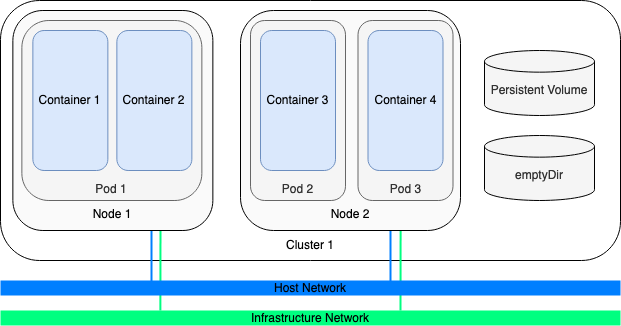
\includegraphics[width=13.5cm]{images/TestArchitectureCluster.png}
    \caption{Kubernetes test cluster overview}
    \label{fig:TestArchitectureCluster}
  \end{center}
\end{figure}

\begin{figure}[ht]
  \begin{center}
    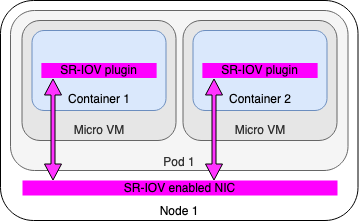
\includegraphics[width=13.5cm]{images/TestArchitectureNode.png}
    \caption{Node test cluster with two containers in a single pod}
    \label{fig:TestArchitectureNode}
  \end{center}
\end{figure}

\subsection{Containers}

The test architecture consists of various relations between containers and storage in a single cluster Kubernetes environment.

Container - container inside pod

Container - container between pods

Container - container across nodes and a pods

Container - storage

\section{Methodology}

The test environment is hosted by a dedicated server which is built and tailored to support edge and far-edge cloud deployments. The server includes X CPU/RAM/Network, which is shared to the cluster. Each test is repeated 10 times, and the results are averaged. The environment is booted between each test to reset the state and possible hanging processes. The system performance is logged with Prometheus/Grafana. The focus in these tests is to measure the possible performance overhead resulting from the Kata Containers and added layer of security.

Mention about using various VMMs (CLH, FC, QEMU compared against runC).

\section{Results}

\subsection{CPU performance}

The architectural design of Kata Containers adds extra components to the system. Each of these components add overhead to the CPU performance via background processes. In the CPU performance tests, the main question was to measure the overhead and the need for extra cores in comparison to runC. The measurement of CPU performance was implemented by creating workloads and recording the performance with Prometheus. 

- CPU overhead of Kata
	- How many cores are needed when Kata is used?
	- From host perspective?
	- Measure
		- Create and delete workloads and record the CPU performance
			- Starting micro-VM might affect the CPU performance
			- Monitor with Prometheus

\subsection{I/O performance}

- Performance of root filesystem
	- Access fs of container
	- Overlay2 fs

- Access to mounted volumes in K8s
	- Create hostPath persistent volume
	- Attach
	- IO

- Attach empty dir to a container
	- Share fs between to containers in a same pod
	- RAM and disk
	- How this is possible?

\subsection{Memory performance}

- Measuring performance of memory not important

- Memory overhead
	- How much the Kata adds to memory used?

\subsection{Storage performance}

- Access to mounted volumes in K8s \\
    - hostPath, emptyDir, local PV \\
	- Create persistent volume \\
	- Attach \\
	- IO \\

\subsection{Network performance}

Networking
    - Evaluate performance \\
    - Two networks. What is the difference?
    - Access to storage not via network, unless NFS(?).

\section{Evaluation}